\documentclass{article}
\usepackage[nonatbib]{project}
\usepackage{watml}

\usepackage[normalem]{ulem}
\usepackage{setspace}
% use Times
\usepackage{times}
% For figures
\usepackage{graphicx} % more modern
%\usepackage{epsfig} % less modern
%\usepackage{subfig} 

% path to figure folder
\graphicspath{{../fig/}}

% bib file for references
\addbibresource{project.bib}


\title{Random Forest Regression Model Feasibility for Plant Data Analysis}

\author{
	Vaaranan Yogalingam \\
	School of Computer Science\\
	University of Waterloo\\
	Waterloo, ON, N2L 3G1 \\
	\texttt{vyogalin@uwaterloo.ca} \\
	{\color{red} report due: August 13}
}

\begin{document}
\maketitle

\begin{abstract} 
This report will discuss the results of experimenting with various models and strategies in determining various plant traits given their images and ancillary data. Ultimately, a random forest regression model led to the best results, seen in this report. The code referenced in this report can be found \href{https://github.com/vaaranan-y/CS480-Final-Project}{here}.
\end{abstract} 

\section{Introduction}
In this report, several methods of predicting the six plant properties (X4,X11,X18,X50,X26,X3112) were explored. Eventually, the highest performing strategy was to use a Random Forest Regressor Model, courtesy of Sci-Kit Learn, trained over the plant trait data, to make the predictions. It was later found that extracting feature vectors from the plant images, using a VGG11 network, courtesy of Pytorch, which combined with the plant trait feature vectors, led to an similarly performing model after a certain number of estimators were used. Such improvement in prediction (as measured by the $R^2$ value) was minimal, with or without image data. This will be explored later on.

\section{Related Works}
Research from multiple works and papers supports the use of a Random Forest Regression Model, for multiple outputs. In this paper on multi-output random forests, two methods of multi-output regression are described. One method would be to use multiple single output regression algorithms, and the other reform the algorithm for multiple outputs. The Random Forest Regressor from SKLearn extends to multi-output problems by leveraging its use of decision trees and averaging over them. There are real world examples of using Random Forests in regression problems, such as in a paper by Hoffman et al. that used Random forest over numerical dust particle information (i.e. size) to predict multiple numerical features of early planet formation. Another example includes a paper by Jog et al., where Random Forests were used to analyze MRI images to address issues of inconsistencies. Unlike these papers that used numerical data and images data separately, this report will briefly explore combining both types of data in the Random Forest model, using a VGG11 network to extract image features (a concept discussed in assignments/lectures).

\section{Main Results}
Two versions of Random Forest were used for experimentation. The first model was fitted solely on the train.csv data provided. In other words no image data was used. In the second model, the image data was incorporated. This was done using feature extraction through the VGG11 model. Below is a table, displaying the score of each random forest model based on the number of estimators and whether or not the model used the image data. Note that the score is based on the coefficient of determination, or $R^2$ value calculated based on 55\% of the data in the public tests.

\begin{table}[H]
\caption{Model Comparison of Random Forest Regressor including and excluding Image Data Respectively (*Note: -- represent the points that could not be recorded due to lack of time for training)}
\begin{tabular}{@{}lcccccc@{}}
\toprule 
\multirow{1}{*}{Number of Estimators} & {Random Forest without Image Data}      & {Random Forest with Image Data}               \\ \midrule                             
100           & 0.19098    & 0.18444                               \\
200        & 0.19529    & 0.18980                          \\
300        & 0.19556           & 0.19443                 \\
400       & 0.19648    & --                           \\
500    & 0.19645           & --               \\
1000    & 0.19714             & 0.19714             \\
\bottomrule
\end{tabular}
\end{table}

This data can also be visualized in a graph like so, in figure one, where the convergence between the model using image data, and the model not using it, is much clearer:

\begin{figure*}[h]
    \centering
    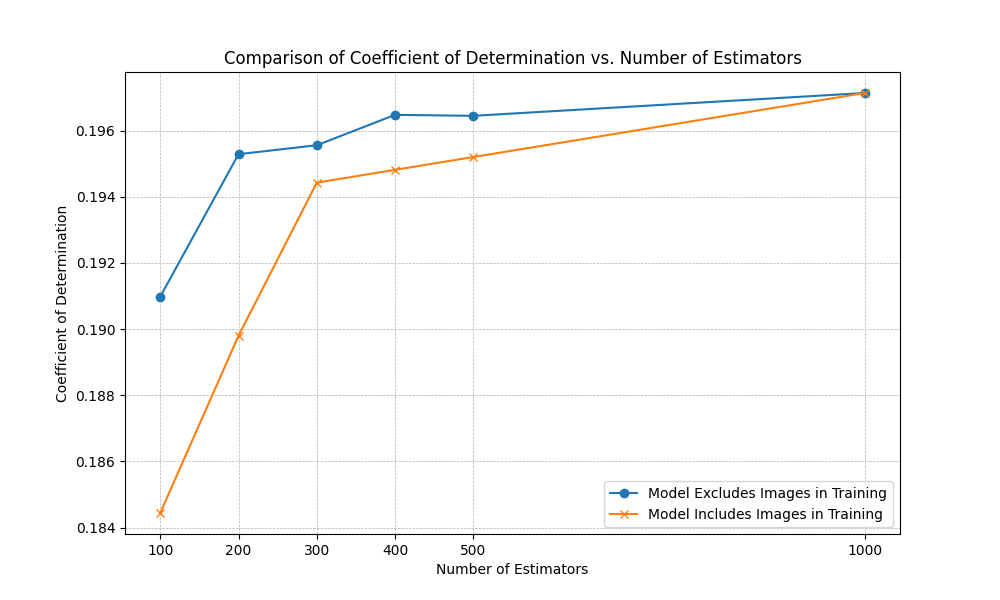
\includegraphics[width=0.9 \textwidth]{PROJECT/Figure_1.png}
    \caption{The progress of the coefficient of determination ($R^2$) as the number of estimators in a Random Forest Regressor model increases. Each line corresponds to when the model does and does not incorporate image data (incorporated via extraction using the VGG11 model). *Note: The model that incorporates the image data in prediction and training, has two interpolated points (at number of estimators being 400 and 500) due to lack of time to complete training.}
    \label{fig:eqv_sde_traj}
\end{figure*}

As can be seen in these models, the greatest jump in the score is from 100 to 200 or 200 to 300 estimators. In general, it would be expected that in any random forest model, that as the number of estimators increases, the measure of accuracy would increase. Increasing the number of estimators, increases the number of trees, which as a bagging algorithm, gives it more data to work off of, but prevents over-fitting, due to how simple these trees are. However, it is worth noticing that while both models eventually converge to approximately the same score (after using 1000 estimators each), the model that uses image data has a lower start, and has consistently large jumps in score between intervals of estimators. Furthermore, some spots are left blank due to a lack of time to run the models with the corresponding number of estimators (as running the model with 1000 estimators took the most time). Both these observations are important in concluding the value of including the image data in training and testing.



\section{Conclusion}
Given the little difference incorporating the image data into the Random Forest regression model made, it is worth questioning when all data is too much data. While similar results were achieved when compared to the model that did not use the image data, the time and energy costs of including image data in the training and testing were probably not worth it. Also, it required a large number of estimators before the model using image data could keep up with the model that did not need that additional data. This could explain why the real world examples mentioned in the introduction of this report, used either image or numerical data, but not both. It would be interesting to explore other possible parameters or methods to make the image data more useful (perhaps through some more complex transformations). Furthermore, perhaps a human analyses of the image would be good to see if they have any relevance to the predicted values (X\_4, X\_11, etc.).

\newpage

\section*{Acknowledgement}
I would like to acknowledge the various sources of documentation I used and referred to when developing my models, including those from Pytorch, Pandas, Pillow, and Scikit Learn, namely Scikit Ensembles, where I was able to retrieve and use the RandomForestRegressor model.
\nocite{*}
\printbibliography[title=References]


\end{document}